\documentclass[conference]{IEEEtran}
\IEEEoverridecommandlockouts
% The preceding line is only needed to identify funding in the first footnote. If that is unneeded, please comment it out.
\usepackage{cite}
\usepackage{amsmath,amssymb,amsfonts}
\usepackage{algorithmic}
\usepackage{graphicx}
\usepackage{textcomp}
\usepackage{xcolor}
\usepackage{hyperref}
\usepackage{amsmath}
\usepackage{amssymb}

\newcommand{\rom}[1]{\uppercase\expandafter{\romannumeral #1\relax}}

\DeclareMathOperator*{\argmin}{arg\,min}

\def\BibTeX{{\rm B\kern-.05em{\sc i\kern-.025em b}\kern-.08em
    T\kern-.1667em\lower.7ex\hbox{E}\kern-.125emX}}
\begin{document}

\title{Assignment 6: a mathematical essay on support vector machine\\}


\author{\IEEEauthorblockN{Gautham Govind A}
\IEEEauthorblockA{\textit{Dept. of Electrical Engineering}\\
\textit{Indian Institute of Technology Madras} \\}
\textit{ee19b022@smail.iitm.ac.in}

}

\maketitle

\begin{abstract}
The objective of this assignment is to explore the mathematical formalism behind support vector machine and then to use it in a real-life application. In this assignment, as a real-life application, support vector machine is used to formally identify how certain features could be used to predict whether a star is a pulsar star or not from the given pulsar star dataset. Data visualization, cleaning and modelling is done using Python. The analysis enables us to arrive at the conclusion that it is possible to make reasonable predictions regarding whether a star is a pulsar or not using simple statistics of the integrated pulse profile and the DM-SNR curve. 
\end{abstract}

\begin{IEEEkeywords}
support vector machine, python, visualization, predictive modelling, binary classification
\end{IEEEkeywords}

\section{Introduction}

Given a set of features and a target variable, predictive modelling is typically used for generating a model which can make predictions for cases where we do not know the value of the target variable, i.e., only the features are available. Apart from this use, a model can also be used for developing an intuition of how various factors influence the target variable. In this assignment, we try to make use of a model for the purpose of identifying the key relationships which influence the decision in a classification problem and then use this model for making predictions.

In particular, we make use of support vector machine (SVM) for the purpose of identifying relationships in a classification problem. Support vector machine is a very robust machine learning algorithm which can be used for tackling both classification and regression problems. Support vector machine is quite popular in the machine learning community because of its strong theoretical framework based on statistical learning theory . Although it is a linear classifier by default, SVMs can efficiently perform a non-linear classification using what is called the kernel trick, implicitly mapping their inputs into high-dimensional feature spaces. This is what makes them really powerful. In our particular problem, we will be using support vector machines for classification.


In our problem setting, the goal is to use support vector machine to predict whether the given star is a pulsar or not given a variety of simple statistics of the integrated pulse profile and the DM-SNR curve. . We make use of a publicly available pulsar star dataset for building the model. After building the model, we evaluate the model using a variety of evaluation metrics. By examining how well the model performs, we can identify how good the identified relationships are. Finally, we make use of our best model to make predictions for cases where the output label is not known,


Section \rom{2} gives an overview of the various techniques used for data cleaning, data visualization and an initial exploratory analysis. A lot of insights can be gained just by making qualitative observations from the given data. Section \rom{3} gives a short description of the mathematical formalism behind support vector machine. Section \rom{4} describes the various models that were tried and the results that were obtained by applying support vector machine in this particular case. Section \rom{5} gives a summary of the major conclusions drawn from the analysis.


\section{Exploratory Data Analysis}

In this section, we describe the process of data cleaning and data visualization. We also make some qualitative observations.

\subsection{Preliminary analysis}

The given dataset has 12528 rows and 9 columns. Eight of the columns form the features, whereas the ninth column is the target variable. We observe that we have \textbf{only continuous variables,} once we exclude the target variable.  

We observe that the eight features are essentially mean, standard deviation, excess kurtosis and skewness of the integrated pulse profile and the DM-SNR curve. A few key points regarding excess kurtosis and skewness:

\begin{itemize}
    \item Kurtosis represents how fat a distribution's tail is when compared to the center of the distribution. 
    \item Excess kurtosis compares the kurtosis coefficient of the distribution with that of a normal distribution. 
    \item Normal distributions have a kurtosis of three. Excess kurtosis can, therefore, be calculated by subtracting kurtosis by three. 
    \item When excess kurtosis is positive, the tails are heavier and when it is negative, tails are thinner than the normal distribution.
    \item Skewness is a measure of degree of asymmetry observed in a probability distribution.
    \item Positive/Right skewed would imply that the mean of the data is greater than the median.
    \item Negative/Left skewed would imply that the mean of the data is less than the median.
\end{itemize}

It also seems that there are null values in three of the features. More precisely, we see that the features 'Excess kurtosis of the integrated profile', 'Standard deviation of the DM-SNR curve' and 'Skewness of the DM-SNR curve'. 

We first plot the non-null values for excess kurtosis of the integrated profile. We obtain a plot as shown in Figure \ref{ktip_bn}. We observe that the tails are rather thin. Hence, we use mean imputing. After imputation, we obtain the plot as shown in Figure \ref{ktip_an}. On plotting the non-null values for standard deviation of DM-SNR curve, we obtain the plot as shown in Figure \ref{stdds_bn}. As the right tail is rather thick, we use median imputation. We obtain the final plot as Figure \ref{stdds_an}. Finally, we look at the plot for skewness of the DM-SNR curve. The plot is shown in Figure \ref{skds_bn}. Again, since the tail is thick we apply median imputation, giving us the plot in Figure \ref{skds_an}.

\begin{figure}[tbh]
\centering
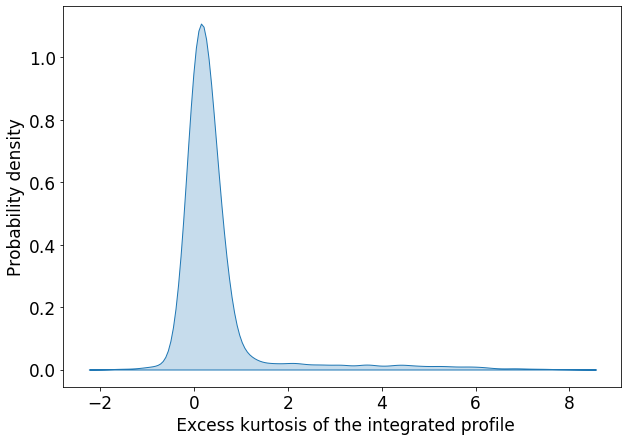
\includegraphics[scale = 0.38]{kip_bn.png}
\caption{Density plot (before imputation - Only non-null values)}
\label{ktip_bn}
\end{figure}

\begin{figure}[tbh]
\centering
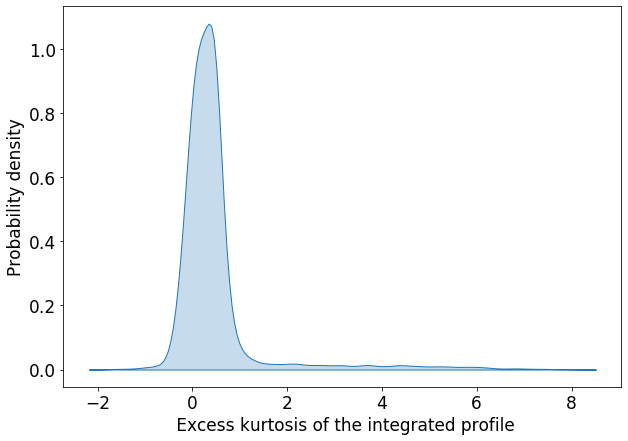
\includegraphics[scale = 0.38]{ktip_an.png}
\caption{Density plot (after imputation)}
\label{ktip_an}
\end{figure}

\begin{figure}[tbh]
\centering
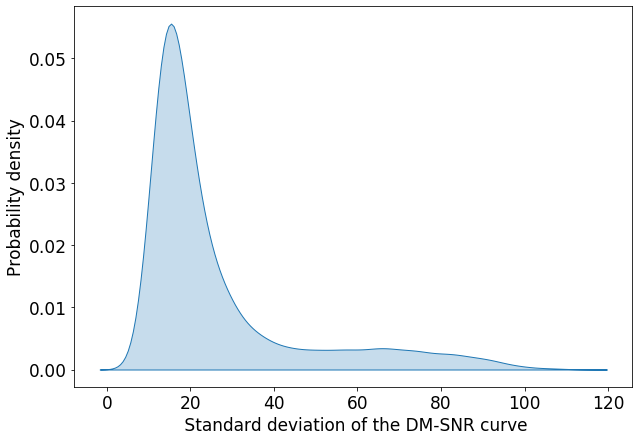
\includegraphics[scale = 0.38]{stdds_bn.png}
\caption{Density plot (before imputation - only non-null values)}
\label{stdds_bn}
\end{figure}

\begin{figure}[tbh]
\centering
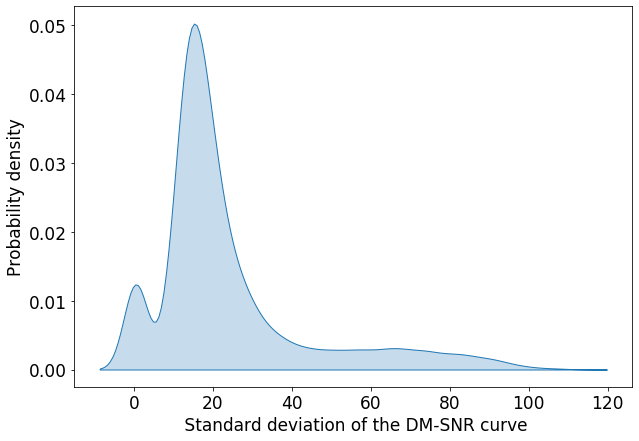
\includegraphics[scale = 0.38]{stdds_an.png}
\caption{Density plot (after imputation)}
\label{stdds_an}
\end{figure}

\begin{figure}[tbh]
\centering
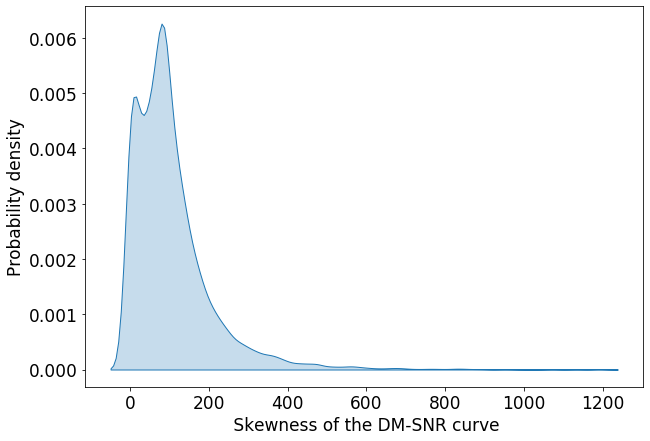
\includegraphics[scale = 0.38]{skds_bn.png}
\caption{Density plot (before imputation - only non-null values)}
\label{skds_bn}
\end{figure}

\begin{figure}[tbh]
\centering
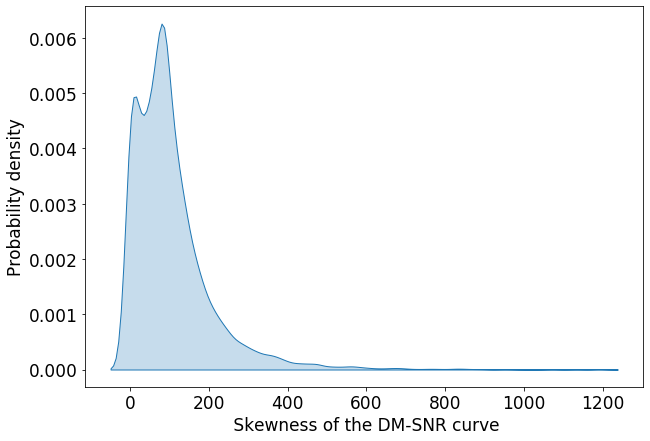
\includegraphics[scale = 0.38]{skds_an.png}
\caption{Density plot (after imputation)}
\label{skds_an}
\end{figure}
 
We also look at the distribution for our target class, which is whether a star is a pulsar or not. On plotting, we obtain Figure \ref{target_dist}. It is observed that only 9.20\% of the total datapoints belong to the class of pulsar stars, implying the dataset is skewed. We will have to account for this during model building.


\begin{figure}[tbh]
\centering
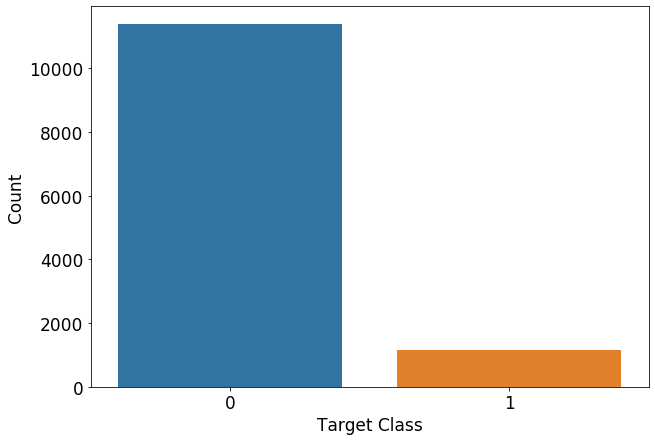
\includegraphics[scale = 0.38]{target_dist.png}
\caption{Target class imbalance}
\label{target_dist}
\end{figure}

\subsection{Feature by feature analysis}

For each feature, we generate a Kernel Density Estimate (KDE) plot, which essentially gives the probability density plot for that particular feature. Moreover, we make the plots separately for stars which are categorized as pulsars and those which are not so as to gain some qualitative idea of how the feature is distributed for the two categories.

The plots for the mean and standard deviation of the integrated profile are shown in Figures \ref{mip_b} and \ref{stdip_b} respectively. \textbf{It can be seen that for stars which are not pulsars, the mean and standard deviation of the integrated profile tend to be higher.} Further, the means of integrated profiles of stars which are pulsars are spread more as compared to non-pulsars. 

\begin{figure}[tbh]
\centering
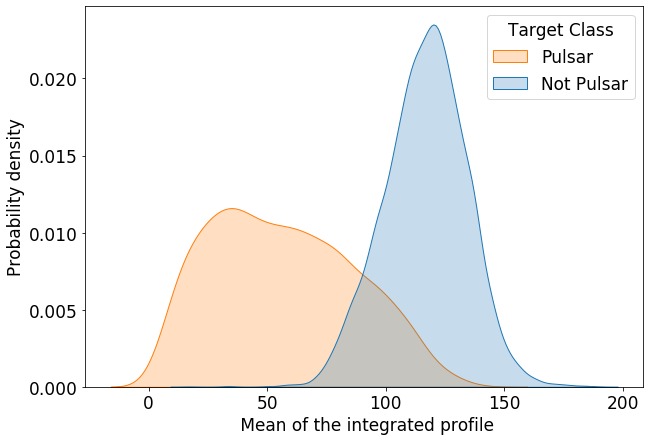
\includegraphics[scale = 0.38]{mip_b.png}
\caption{Density plot for mean of integrated profile}
\label{mip_b}
\end{figure}

\begin{figure}[tbh]
\centering
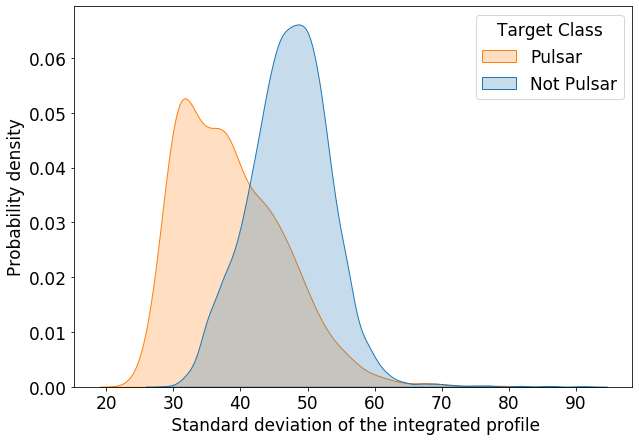
\includegraphics[scale = 0.38]{stdip_b.png}
\caption{Density plot for standard deviation of integrated profile}
\label{stdip_b}
\end{figure}

The plots for the excess kurtosis and skewness of the integrated profile are shown in Figures \ref{kip_b} and \ref{skip_b} respectively. \textbf{In both cases, the distribution is more spread out for stars which are pulsars.}

\begin{figure}[tbh]
\centering
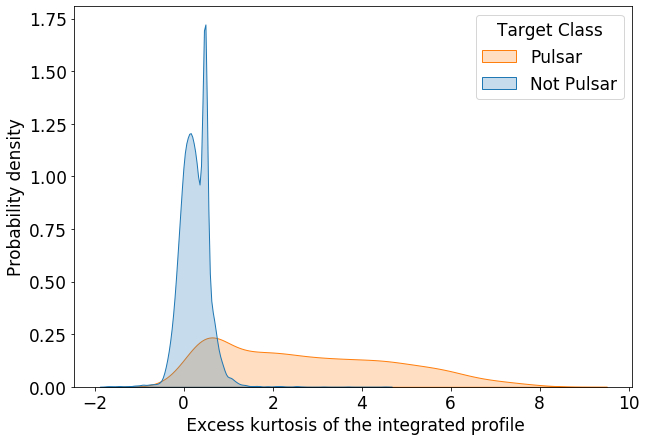
\includegraphics[scale = 0.38]{ktip_b.png}
\caption{Density plot for excess kurtosis of integrated profile}
\label{kip_b}
\end{figure}

\begin{figure}[tbh]
\centering
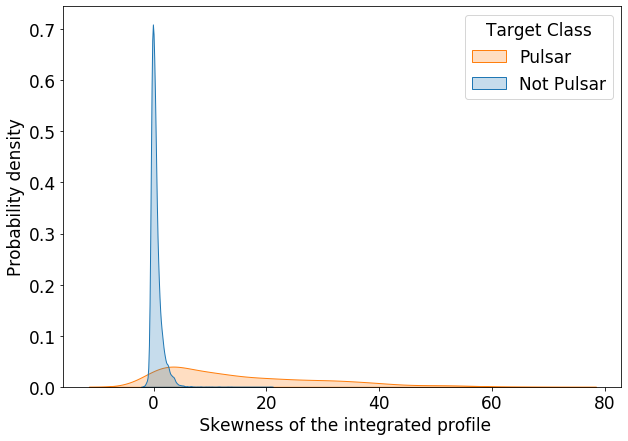
\includegraphics[scale = 0.38]{skip_b.png}
\caption{Density plot for skewness of integrated profile}
\label{skip_b}
\end{figure}


The plots for the mean and standard deviation of the DM-SNR curve are shown in Figures \ref{mds_b} and \ref{stdds_b} respectively. \textbf{It can be seen that for stars which are  pulsars, the mean and standard deviation of the DM-SNR curve tend to be higher.} Further, the means and standard deviations of DM-SNR curves of stars which are pulsars are spread more as compared to non-pulsars. 

\begin{figure}[tbh]
\centering
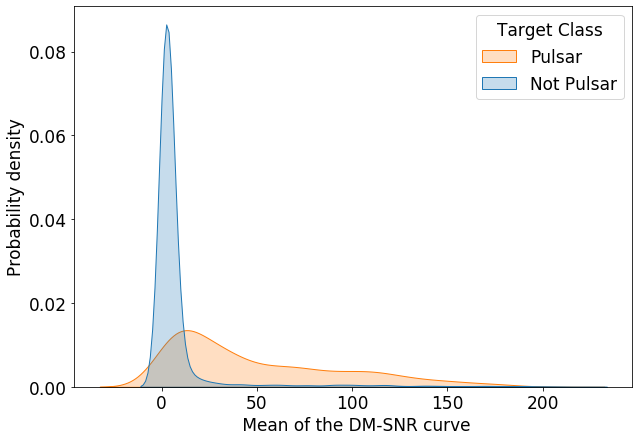
\includegraphics[scale = 0.38]{mds_b.png}
\caption{Density plot for mean of DM-SNR curve}
\label{mds_b}
\end{figure}

\begin{figure}[tbh]
\centering
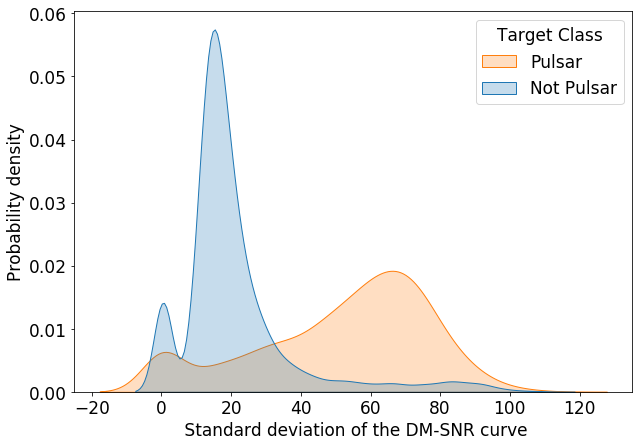
\includegraphics[scale = 0.38]{stdds_b.png}
\caption{Density plot for standard deviation of DM-SNR curve}
\label{stdds_b}
\end{figure}

The plots for the excess kurtosis and skewness of the DM-SNR curve are shown in Figures \ref{ktds_b} and \ref{skds_b} respectively. \textbf{In both cases, the distribution is more spread out for stars which are not pulsars.}

\begin{figure}[tbh]
\centering
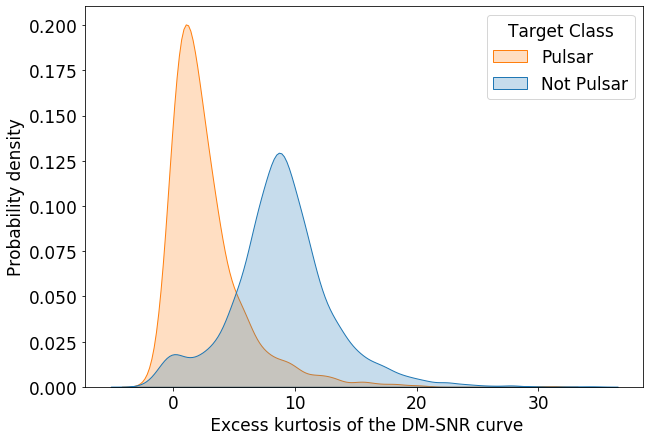
\includegraphics[scale = 0.38]{ktds_b.png}
\caption{Density plot for excess kurtosis of DM-SNR curve}
\label{ktds_b}
\end{figure}

\begin{figure}[tbh]
\centering
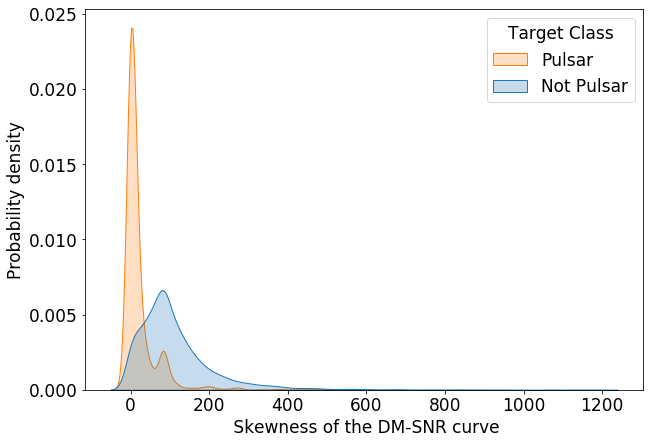
\includegraphics[scale = 0.38]{skds_b.png}
\caption{Density plot for skewness of DM-SNR curve}
\label{skds_b}
\end{figure}


\section{Model: Support Vector Machine}

In this section, we will give a brief overview of the mathematical formalism behind the support vector classifier. 

Support vector machines in general support both regression and classification. The classifier based on the principle of support vector machines is often referred to as support vector classifiers. By default, SVM is designed for the case of binary classification. Extension to multinomial classification is non-trivial and is not of interest to us currently. Also, SVM without any modification is a linear classifier. However, it is possible to introduce non-linearities through the 'kernel' trick which we will get to very soon.

SVMs follow a discriminant modelling approach, which means that the model directly maps each sample to a class instead of assigning class probabilities. This is in contrast with generative models like logistic regression and naive bayes which rely on computation of posterior probabilities for assigning class labels.

The support vector machine is a generalization of a simple and intuitive classifier called the maximal margin classifier. The main issue with the vanilla maximal margin classifier is that it requires the dataset to be strictly linearly separable which is a rather unreasonable requirement. SVM is an extension of maximal margin classifier which relaxes this requirement. We explore these concepts more rigorously in the following sections.

\subsection{Maximal margin classifier}

Before introducing the maximal margin classifier, it is necessary to understand what a hyperplane is. A hyperplane is a subspace of one dimension less than of its ambient space. Intuitively, it can be thought of as an extension of a line in X-Y plane or a plane in X-Y-Z plane to arbitrarily higher number of dimensions. Mathematically, a hyperplane in a p-dimensional space is governed by an equation of the form:

$$ f(\mathbf{X}) = w_1x_1 + w_2x_2 ... + w_px_p + b = 0 $$

Suppose we have a dataset with $n$ datapoints with each datapoint having $p$ features each. If we assume the labels to be $y_i = \{-1, +1\}$, then for the dataset to be linearly separable,
$$ f(\mathbf{X}) > 0 \hspace{0.2cm} \textrm{if } y_i = +1  $$
$$ f(\mathbf{X}) < 0 \hspace{0.2cm} \textrm{if } y_i = -1  $$

This can be rewritten as:
$$ y_if(\mathbf{X}) > 0 $$
$$ y_i(w_1x_1 + w_2x_2 ... + w_px_p + b) > 0 $$

The condition which we have derived so far is the condition necessary for the dataset to be considered linearly separable. Now, if we know a given dataset is linearly separable, it is possible to draw several lines separating the two classes. How do we decide which line is the best?

An intuitive answer is to take the line with the largest margin, which is essentially the distance to the closest point. This strategy is what is called maximal margin classification. A key feature of maximal margin classifiers are support vectors. Essentially, the position and slope of the line is determined only by those points which are closest to the line. If these points were to shift around slightly, the line would get shifted, whereas changing points other than the supports would have no effect on the line whatsoever.

Mathematically, this can be stated as:
\begin{equation*}
    \max_{w, b} \min_{i \in n} \frac{|w^Tx_i + b|}{||w||} 
\end{equation*}
\begin{equation*}
    \textrm{s.t. sign}(w^Tx_i + b) = y_i
\end{equation*}

After some mathematical manipulations, it can be shown that the above maximization is equivalent to the following minimization:
\begin{equation*}
    \min_{w. b} \frac{1}{2}{||w||^2} 
\end{equation*}
\begin{equation*}
    \textrm{s.t. }y_i(w^Tx_i + b) \geq 1
\end{equation*}

\subsection{Soft margin classifier}

As stated earlier, the maximal margin classifier is not ideal since it enforces linear separability, which is not compatible with most of the real-life datasets. In order to obtain a greater robustness
we aim to modify the classifier to work in situations where a majority of the points are separable whereas a small fraction is not. This is the principle behind support vector classifier also known as the soft margin classifier.

The classifier is called soft margin because the separability condition can be violated by some of the training observations. Rather than seeking the largest possible margin so that every observation is not only on the correct side of the hyperplane but also outside the margin, we instead allow some observations to be inside the margin or even on the incorrect side of the hyperplane. The points that fall on the incorrect side of the hyperplane are miss-classified. These points together with those that fall within and on the margin are the support vectors of the classifier that influence the decision boundary.

To make things more concrete mathematically, let us define the slack variable $\epsilon _i$. If a datapoint $X_i$ falls outside the margin, $\epsilon _i = 0$, whereas $\epsilon _i > 0$ for support vectors. The soft-margin problem could then be written as:

\begin{equation*}
    \min_{w. b} \hspace{0.3cm} \frac{1}{2}{||w||^2} + C\sum_{i=1}^{n}\epsilon _i
\end{equation*}
\begin{equation*}
    \textrm{s.t. } \hspace{0.2cm} y_i(w^Tx_i + b) \geq 1 - \epsilon _i
\end{equation*}
\begin{equation*}
    \epsilon _i \geq 0
\end{equation*}

The hyperparameter $C$ determines the severity of the violations to the margin. If $C \rightarrow \infty$, the cost associated for miss-classification is very high and thence results resemble that of a hard-margin classifier. If $C$ is very less, we allow more observations to violate the margin, hence also allowing more miss-classifications.

In practice, $C$ is treated as tuning parameter that is chosen via cross validation. When $C$ is large, we seek narrow margins that are rarely violated. This amounts to a classifier that is highly fit to data, hence may have low bias but high variance. On the other hand, when $C$ is small, the margin is wider, and we allow more violations to it. This amounts to fitting the data less forcefully and obtaining a classifier that is potentially more biased but has a lower variance. Hence we can say that $C$ controls bias-variance trade-off.

\subsection{Solution to the optimization problem}

The Lagrangian of the soft margin classifier optimization problem in the primal space can be written as:

\begin{align*}
  L(w, b, \epsilon, \alpha, \beta) = \frac{1}{2}{||w||^2} + C\sum_{i=1}^{n}\epsilon _i + \sum_{i=1}^{n}\beta_i(-\epsilon _i) + \\
  \sum_{i=1}^{n}\alpha_i(1 - \epsilon _i - y_i(w^Tx_i + b)) 
\end{align*}

where $\alpha_i$ and $\beta_i$ are lagrange multipliers and hence are non-negative. The above problem can be solved in the dual space by applying min-max theorem. Though the solution process is a bit complicated, the result of this optimization is interesting. The decision function obtained is:

$$ f(x) = \beta_0 + \sum_{i = 1}^n\alpha_i <x, x_i> $$

where $< x, x_i >$ is dot product and $\alpha_i \neq 0$ for support vectors only. Since the decision boundary is only dependent on support vectors, SVM is quite robust to behavior of observations that are far away (outliers) from the hyperplane.

\subsection{Kernel Trick}

Since the decision function depends on dot product of support vectors only, we can rewrite the decision function as:

$$ f(x) = \beta_0 + \sum_{i = 1}^n\alpha_i K(x, x_i) $$

where $K(x, x_i)$ represents the dot product in some higher dimensional plane. The intuition behind this is that we now would be able to achieve the effect of transforming X to a higher dimensional subspace without actually performing the transformation. This is because we effectively need only the dot product which can be computed using functions called kernels, which is denoted by K here.A kernel essentially is a transformation to a higher dimensional subspace through dot products without performing the transformation directly. This is advantageous computationally. The following are popular choices of kernel:

\begin{itemize}
    \item $K(x_i, x_j) = x_i^Tx_j$: Linear kernel (no transformation).
    \item $K(x_i, x_j) = (1+x_i^Tx_j)^d$: Polynomial kernel (Transformation into polynomial space of degree d).
    \item $K(x_i, x_j) = \textrm{exp}(-\gamma||x_i-x_j||^2)$: RBF Kernel. (Transformation into infinite-dimensional Hilbert Space).
\end{itemize}

\section{Modelling }

In this section, we discuss the application of the support vector classifier to our problem. 

We create and evaluate multiple models based on the following hyperparameters:

\begin{itemize}
    \item \textbf{Kernel:} We try SVC classifiers with linear and rbf kernels.
    \item \textbf{C:} C here is the hyperparameter which was discussed during discussion of soft-margin classifier.
    \item $\mathbf{\gamma}$: $\gamma$ is a hyperparameter applicable only for the case of rbf kernel. This hyperparameter helps tune the amount of regularization.
\end{itemize}

We also define each SVC classifier such that appropriate class weights are assigned to each of the target class, such that the imbalance in the dataset is accounted for.

We evaluate the models based on multiple metrics. A short description of the metrics used is given below:

\begin{itemize}
    \item \textbf{Accuracy:}
    Accuracy is simply the \textbf{ratio of number of correct predictions to total number of predictions.} Although this seems like a very good metric intuitively, accuracy fails on classification problems with a skewed class distribution because of the intuitions developed by practitioners on datasets with an equal class distribution.
    \item \textbf{Precision:}
    Precision is the \textbf{ratio of true positives to the total positive predictions.} Precision is typically used when the cost of false positive is high. For instance, email spam detection.
    \item \textbf{Recall:}
    Precision is the \textbf{ratio of true positives to the total positive ground truths.} Recall is typically used when the cost of false negative is high. For instance, in fraud detection or sick patient detection.
    \item \textbf{F1-score:}
    F1-score is simply a \textbf{harmonic average of precision and recall.} F1 Score is typically used if we need to seek a balance between Precision and Recall and there is an uneven class distribution.
    
    
\end{itemize}


We will be using \textbf{f1-score} as the metric for comparison between models. The dataset is split into training and validation sets. The test set, which has been provided separately, is kept aside and will be used only after choosing the best model. Comparison between models is done using validation set.

After performing a grid search over the hyperparameter space and comparing multiple different models through cross-validation, we arrive at the conclusion that for the given dataset, the best set of hyperparameters are \textbf{kernel = rbf, C = 5.039 and }$\mathbf{\gamma = 0.231}$. The best model has 1090 support vectors for class 0 and 224 support vectors for class 1. \textbf{This means that out of the total 8769 samples, only 1314 are support vectors.} This goes to show that only a small fraction of the points actually contribute to the SVM decision boundary.

The confusion matrix for the best model is shown in Figure \ref{conf_mat}. The values for the evaluation metrics are given in Table \ref{met}.

\begin{figure}[tbh]
\centering
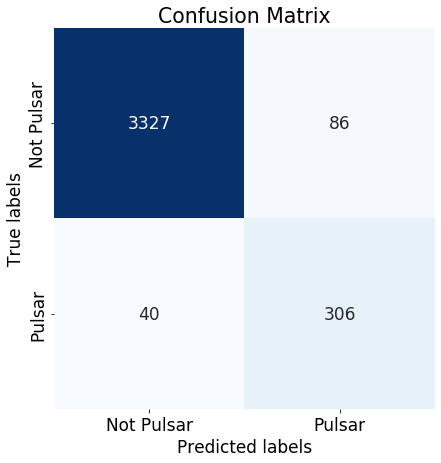
\includegraphics[scale = 0.38]{conf_mat.png}
\caption{Confusion matrix for the best model}
\label{conf_mat}
\end{figure}

\begin{table}
\begin{center}

\caption{Metrics for the best model}

\begin{tabular}{| c| c| }
 \hline
 Metric & Score \\
 \hline
 \hline
 Accuracy & 0.966 \\ 
 \hline
 Precision & 0.781 \\   
 \hline
 Recall & 0.884 \\
 \hline
 F1 Score & 0.829 \\
 \hline

\end{tabular}

\label{met}
\end{center}

\end{table}

ROC curve is another common tool used with binary classifiers. A Receiver Operating Characteristic curve, or ROC curve, is a graphical plot that illustrates the diagnostic ability of a binary classifier system as its discrimination threshold is varied. The ROC curve is created by plotting the true positive rate (TPR) against the false positive rate (FPR) at various threshold settings. The ROC curve for our model is given in Figure \ref{Rocauccurve}.

\begin{figure}[tbh]
\centering
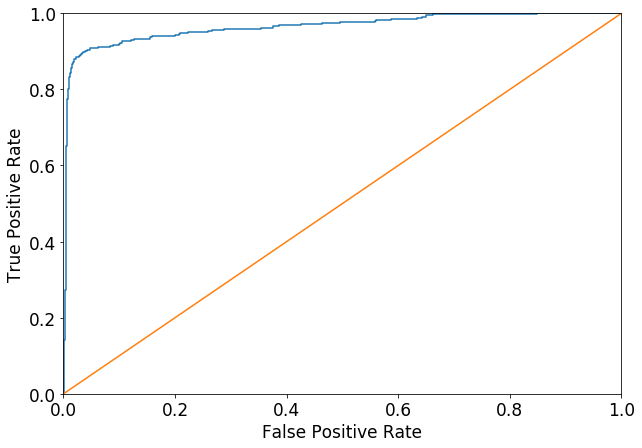
\includegraphics[scale = 0.38]{Rocauccurve.png}
\caption{ROC curve for the best model}
\label{Rocauccurve}
\end{figure}

The dotted line represents the ROC curve of a purely random classifier; a good classifier stays as far away from that line as possible (toward the top-left corner). One way to compare classifiers is to measure the area under the curve (AUC). A perfect classifier will have a ROC AUC equal to 1, whereas a purely random classifier will have a ROC AUC equal to 0.5. \textbf{The area under the ROC curve of our classifier is 0.964.}

Note that the standard ROC Curve requires varying the probability of score threshold of a classifier and obtaining the corresponding graph of the ordered pairs (TPR,FPR) for
each threshold. But since SVM is defined in a such a way that it doesn't produce probabilities directly, we can only approximate these by computing signed distance between the hyperplane and the points. So the above is only an estimate of the ROC curve.

Finally, predictions were also made for the best model that was obtained on the given test dataset.


\section{Conclusions}

From our extensive analysis of the given dataset using support vector classifier, we arrive at the following conclusions:

\begin{itemize}
    \item Support vector machines are robust algorithms which are. in comparison. less sensitive to outliers than most of the other popular algorithms.
    \item Usage of the kernel trick is a clever way to search in higher dimensional space without increasing computational complexity.
    \item Accuracy may not be a good measure of performance for imbalanced classification tasks. It is necessary to use metrics like weighted f1-score for such cases.
    \item Best performance is obtained by setting kernel as rbf, C = 5.039 and $\gamma = 0.231$.
    \item A good fit is obtained for the model, meaning whether a star is a pulsar or not can be predicted to a very good extent from simple statistics of integrated profile and DM-SNR curve.
\end{itemize}



\section{Avenues for further research}

Support vector performs quite well for the given dataset. Doing some kind of feature preprocessing like PCA, to extract important features before inputting it to the model might help. Extracting more statistics while preparing the dataset itself will help improve model performance.  



\nocite{*} % Print all references regardless of whether they were cited in the poster or not
\bibliographystyle{ieeetr}
\bibliography{sample} % Use the example bibliography file sample.bib


\end{document}

